\section{Implementation and evaluation}
\label{sec:experiments}
We implement the dispute resolution protocol using the \pytorch framework (version 2.4), with neural network models defined as \onnx computational graphs~\cite{onnx2017}, 
and we implement the \repops library using the \cuda framework (version 12.1). 
\footnote{
A demo of \repops showing reproducibility on certain Llama models 
on CPU and GPU 
is available at \url{https://github.com/gensyn-ai/repop-demo}. 
We're also working on developing \repops into a Python module.
}

This section describe our benchmarks of \repops, focusing on its relative overhead versus 
\pytorch using the hardware-optimized implementations of 
operators from the \cudnn library. 
We test on four GPUs with varying amount of VRAM in our experiments, all from Nvidia: 
T4 (16 GB), RTX 3090 (24 GB), A100 (40 GB variant), and 
A100 (80 GB variant). 
Our \repops implementation currently supports FP32, as that had the most 
widespread \ieeefp compliance support. 

For each experiment, we state our main observations and 
  extract key patterns that shed light on operator performance 
  and indicates directions to take for real-world deployment of \repops. 
We note that the code underlying \cudnn
  is closed-source, and thus we do not have access to all the optimizations 
  they use, nor can we add our own optimizations. 

\subsection{Matrix multiplication.}
\label{sec:matmul-microbenchmarks}
Matrix multiplication is by far the most prevalent and expensive operation in 
  neural networks, making it a key factor for end-to-end model performance. 
We benchmark the \repops matrix multiplication overhead 
  for various dimensions, 
  comparing it against the \pytorch and \cudnn implementation 
  (i.e., \texttt{torch::mm}). 
For each dimension and hardware pairing, 
we explore a wide array of kernel parameters, 
including elements of the final matrix per thread, tile size, and block sizes, 
and  report the performance of the best one. 
Figure~\ref{fig:matmul_microbenchmarks} shows our results for two GPUs 
emblematic of the general trend we observe. 

\begin{figure}[t]
    \centering
    \resizebox{\columnwidth}{!}{


\pgfplotsset{compat=1.18}

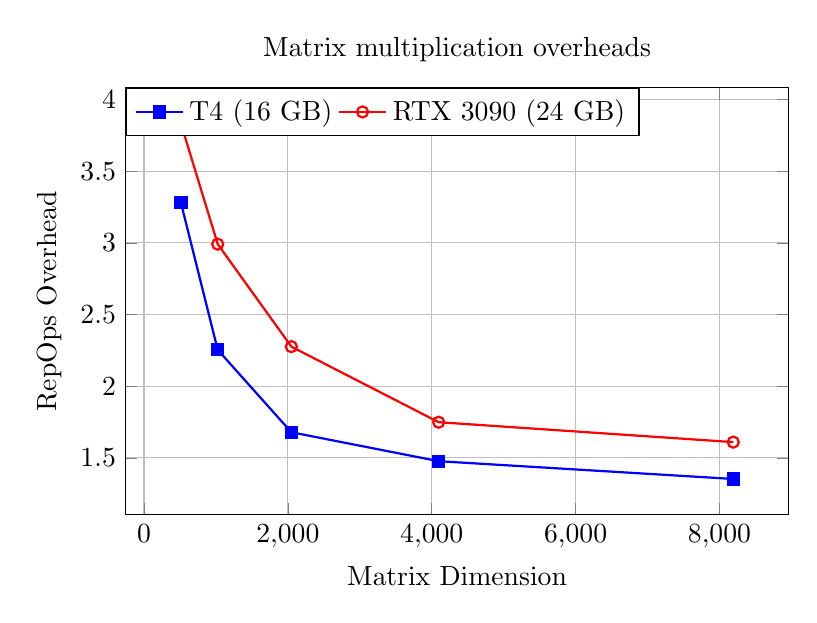
\begin{tikzpicture}
\begin{axis}[
    width=10cm, %
    height=7cm, %
    xlabel={Matrix Dimension}, %
    ylabel={RepOps Overhead}, %
    grid=both, %
    legend style={at={(0,1)}, anchor=north west, legend columns=2},
    title={Matrix multiplication overheads},
    extra y ticks={0},
extra y tick style={
  grid=major,
  major grid style={dashed,line width=0.5pt, black}
}
]

\addplot[
    color=blue, 
    mark=square*, 
    thick
]
coordinates {
    (512, 3.281)
    (1024, 2.254)
    (2048, 1.679)
    (4096, 1.477)
    (8192, 1.353)
};

 

\addplot[
    color=red, 
    mark=o, 
    thick
] 
coordinates {
    (512, 3.833)
    (1024, 2.991)
    (2048, 2.276)
    (4096, 1.749)
    (8192, 1.610)
};


\legend{T4 (16 GB), RTX 3090 (24 GB)}
\end{axis}
\end{tikzpicture}



}
\caption{\repops overhead for matrix-matrix multiplication.}
    \label{fig:matmul_microbenchmarks}
\end{figure}

\uline{Observation 1: \repops matrix multiplication overhead improves significantly 
with the matrix size.}

The amount of parallelization ``left on the table'' by \repops 
is more significant when the total amount of computation to be done is less, 
as is the case when the matrices are smaller. 
In other words, as matrices grow larger the parallelization performed in \repops 
is enough for better utilization of the GPU's resources. 
This leads to a sort of steady state overhead of 60\%-70\% for RTX 3090 (24 GB) 
and about 35\% for T4 (16 GB).









\subsection{Model inference and training benchmarks.}

We measure the performance of three models, \distilbert (66 million parameters), 
\llama-3.1-1B, and \llama-3.1-8B.
Table~\ref{table:repops_models} shows the average overhead on inference and training tasks 
for the first two models, 
and Table~\ref{table:repops_llama_8b} shows that of inference and fine-tuning tasks for the last
(as our GPUs did not have enough memory to train an 8 billion parameter 
model in FP32). 
We use the Adam optimizer for both training and fine-tuning.
As before, all programs are run in FP32.
We tested on various input shapes and sequence lengths and found the overheads 
obtained to be similar in all settings. 
We tested all training benchmarks on batch sizes from 2 to 8 and
found similar numbers for all benchmarks 
(we show the \emph{worst} performing batch size for each).
We note that the overheads of the \llama models slightly \emph{decreased} as we increase 
the batch size.

\begin{table}[t]
\centering
\caption{\repops training and inference overheads for \distilbert and \llama-1B.}
\label{table:repops_models}
\begin{tabular}{lrrrr}
\toprule
\textbf{Hardware} & \multicolumn{2}{c}{\textbf{\distilbert}} & \multicolumn{2}{c}{\textbf{\llama-1B}} \\
 & \textbf{Infer.} & \textbf{Train.} & \textbf{Infer.} & \textbf{Train.} \\
\midrule
T4 (16 GB)   & 74\% & 258\%  & 218\%  & 374\% \\
A100 (40 GB) & 84\%  & 312\%  & 58\%  & 67\% \\
\end{tabular}
\end{table}

\begin{table}[t]
\centering
\caption{\repops overheads for \llama-8B.}
\begin{tabular}{lcc}
  \toprule 
\textbf{Hardware} & \textbf{Inference} & \textbf{Fine-tuning (LoRA)}   \\
\midrule
A100 (80 GB)   &  98\% & 126\% \\
\end{tabular}
\label{table:repops_llama_8b}
\end{table}



\uline{Observation 2: \repops performs relatively much better on the larger \llama models 
than the smaller \distilbert.}

Analogous to how smaller matrix multiplications incur higher overheads, 
the \distilbert models being less compute intensive accentuates 
the impact of the limited parallelism of \repops. 
Another issue is that \distilbert performs many operators like LayerNorm, GeLU, 
and ERF that are not present in \llama, which we did not focus on optimizing. 

\uline{Observation 3: \llama overheads are significantly better 
in the larger memory (40 GB VRAM) and bandwidth GPU than the smaller memory (16 GB VRAM)
and bandwidth one.}
With memory management being less of a concern, 
larger GPUs see less of the performance issues related to memory transfers as opposed to smaller GPUs. 
Since RepOps as a backend does not tend to allocate excess memory, 
it would make sense that the performance benefits related to larger GPU memory apply not just 
for Torch's runtime but also \repops's. 
This becomes an outsized factor when using larger models with over 1 billion parameters. 




